\documentclass{standalone}
\usepackage{tikz}
\begin{document}


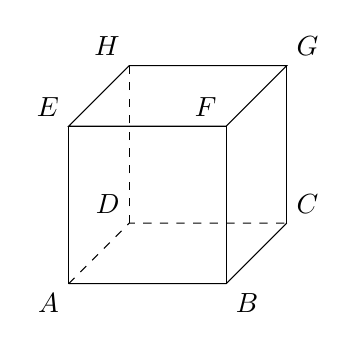
\begin{tikzpicture}[scale=2]
    % 定义立方体的顶点
    \coordinate (A) at (0,0,1);
    \coordinate (B) at (1,0,1);
    \coordinate (C) at (1,0,0);
    \coordinate (D) at (0,0,0);
    \coordinate (H) at (0,1,0);
    \coordinate (G) at (1,1,0);
    \coordinate (F) at (1,1,1);
    \coordinate (E) at (0,1,1);
    % 绘制底面
    \draw (A) -- (B) -- (C);
    \draw[dashed]  (A) -- (D) -- (C);
    % 绘制顶面
    \draw (E) -- (F) -- (G) -- (H) -- cycle;
    % 绘制侧面
    \draw (A) -- (E);
    \draw[dashed] (D) -- (H);
    \draw (B) -- (F);
    \draw (C) -- (G);
    % 标注顶点
    \node[below left] at (A) {$A$};
    \node[below right] at (B) {$B$};
    \node[above right] at (C) {$C$};
    \node[above left] at (D) {$D$};
    \node[above left] at (E) {$E$};
    \node[above left] at (F) {$F$};
    \node[above right] at (G) {$G$};
    \node[above left] at (H) {$H$};
\end{tikzpicture}

\end{document}


% convert -density 300 正方体.pdf 正方体.png
